%
% main.tex -- Paper zum Thema <autotune>
%
% (c) 2020 Autor, OST Ostschweizer Fachhochschule
%
% !TEX root = ../../buch.tex
% !TEX encoding = UTF-8
%
\chapter{Thema\label{chapter:autotune}}
\kopflinks{Thema}
\begin{refsection}
\chapterauthor{Hans Muster}

Ein paar Hinweise für die korrekte Formatierung des Textes
\begin{itemize}
\item
Absätze werden gebildet, indem man eine Leerzeile einfügt.
Die Verwendung von \verb+\\+ ist nur in Tabellen und Arrays gestattet.
\item
Die explizite Platzierung von Bildern ist nicht erlaubt, entsprechende
Optionen werden gelöscht. 
Verwenden Sie Labels und Verweise, um auf Bilder hinzuweisen.
\item
Beginnen Sie jeden Satz auf einer neuen Zeile. 
Damit ermöglichen Sie dem Versionsverwaltungssysteme, Änderungen
in verschiedenen Sätzen von verschiedenen Autoren ohne Konflikt 
anzuwenden.
\item 
Bilden Sie auch für Formeln kurze Zeilen, einerseits der besseren
Übersicht wegen, aber auch um GIT die Arbeit zu erleichtern.
\end{itemize}

%
% teil1.tex -- Beispiel-File für das Paper
%
% (c) 2020 Prof Dr Andreas Müller, Hochschule Rapperswil
%
% !TEX root = ../../buch.tex
% !TEX encoding = UTF-8
%
\section{Einführung in das Verhalten eines Strahls
	\label{ct:section:EinführungEinesStrahls}}
\rhead{Einführung in das Verhalten eines Strahls}

Im vorliegenden Abschnitt wird das Verhalten eines Strahls erklärt. Um die Analyse zu vereinfachen, werden bestimmte Annahmen getroffen, damit eine idealisierte Sichtweise der Röntgenstrahlen und ihres Verhaltens darzustellen. Diese Annahmen werden im folgenden Abschnitt beschrieben.

\subsection{Annahmen eines Röntgenstrahls
	\label{ct:subsection:annahmen}}
In erster Linie betrachten wir einen Röntgenstrahl als eine Zusammensetzung von Photonen und nehmen an, dass er monochromatische Eigenschaften aufweist. Diese monochromatische Eigenschaft bedeutet, dass alle Photonen dieselbe Energie $E$ besitzen und mit einer konstanten Frequenz propagieren. $N(x)$ steht für die Anzahl der Photonen pro Sekunde, die einen bestimmten Punkt $x$ durchqueren. Somit kann die Intensität des Strahls an einem Punkt $x$ mit
\begin{equation}
	I(x) = E\cdot N(x)
\end{equation}
beschrieben werden. Darüber hinaus gehen wir davon aus, dass Röntgenstrahlen eine vernachlässigbare Breite haben und von Brechung oder Beugung unbeeinflusst bleiben. Das bedeutet, dass die Röntgenstrahlen bei der Ausbreitung durch ein Medium weder gebogen noch gestreut werden.

Jede Substanz hat die Eigenschaft, beim Durchgang von Röntgenstrahlen pro Millimeter einen bestimmten Anteil an Photonen zu absorbieren. Dieser einzigartige substanzabhängige Anteil wird als Dämpfungskoeffizient bezeichnet. Die Einheit des Dämpfungskoeffizienten kann auf eine Art beschrieben werden, als \glqq wie viele Photonen werden pro Millimeter des Mediums absorbiert\grqq. Dieser Dämpfungskoeffizient ist im Allgemeinen ein positiver Wert und ist vom Material abhängig.  
\begin{table}
	\centering
	\begin{tabular}{|>{}c<{}|>{}c<{}| >{}c<{}| >{}c<{}|}
		\hline
		Medium &  Hounsfield Einheit & Medium &  Hounsfield Einheit\\
		\hline
		Knochen & 1000		& Niere & 30\\
		Leber 	& 40 bis 60	& Gehirn-Rückenmarks-Flüssigkeit & 15\\
		Blut 	& 40		& Wasser & 0\\
		Muskel 	& 10 bis 40 & Luft & -1000\\
		\hline
	\end{tabular}
	\caption{Ungefähre Hounsfield Einheiten für verschiedene organische Substanzen.
		\label{ct:hounsfieldunits}}
\end{table}

In der Praxis verwenden Radiologen eine modifizierte Version des Dämpfungskoeffizienten, die sogenannte Hounsfield-Einheit. Dieser von Godfrey Hounsfield eingeführte Zahlenwert ermöglicht einen direkten Vergleich zwischen dem Abschwächungskoeffizienten eines Mediums und dem von Wasser. Die Hounsfield-Einheit eines Mediums ist
\begin{equation}
	H_{\textbf{Medium}} := \dfrac{A_{\textbf{Medium}}-A_{\textbf{Wasser}}}{A_{\textbf{Wasser}}},
\end{equation}
wobei $A$ der wahre Dämpfungskoeffizient ist. In der Tabelle \ref{ct:hounsfieldunits} werden verschiedene Hounsfield Einheiten für organische Substanzen aufgelistet.

Ein Röntgenstrahl durchquert ein Medium zwischen zwei Punkten $x$ und $x + \Delta x$. $A(x)$ sei der Dämpfungskoeffizient dieses Mediums an diesem Ort. In diesem Fall ist der Anteil der Photonen, die innerhalb des Intervalls $[x, x + \Delta x]$ absorbiert werden, durch $p(x) = A(x)\Delta x$ gegeben. Die Anzahl der vom Medium in diesem Intervall absorbierten Photonen pro Sekunde lässt sich folglich ausdrücken als $p(x) \cdot N(x) = A(x) \cdot N(x) \cdot \Delta x$. Werden beide Seiten mit der Energie $E$ jedes Photons multipliziert, so kann festgestellt werden, dass dies dem Intensitätsverlust des Röntgenstrahls in dem genannten Intervall entspricht. Dieser Intensitätsverlust kann mit 
\begin{equation}
	\Delta I \approx -A(x) \cdot I(x) \cdot \Delta x
\end{equation}
ausgedrückt werden.

Beers Gesetz ist die daraus folgende Differentialgleichung, die resultiert, wenn $\Delta x \rightarrow 0$, wobei 
\begin{equation}
	\dfrac{dI}{dx} = -A(x)\cdot I(x).
\end{equation}
Das beersche Gesetz beschreibt die Änderung der Intensität pro Millimeter eines nicht brechenden, monochromatischen, null-breiten Röntgenstrahls, der ein Medium durchquert, welche direkt proportional sowohl zur Intensität des Strahls als auch zum Dämpfungskoeffizienten des Mediums ist.

Diese Differentialgleichung ist separierbar und kann auch geschrieben werden als
\begin{equation}
	\dfrac{dI}{I} = -A(x)\,dx.
\end{equation}
Wenn der Strahl am Ort $x_0$ mit einer anfänglichen Intensität von $I_0 = I(x_0)$ beginnt und nach dem Durchgang durch das Medium am Ort $x_1$ mit einer endgültigen Intensität von $I_1 = I(x_1)$ detektiert wird, ergibt sich 
\begin{equation}
	\int_{x_0}^{x_1} \dfrac{dI}{I} = -\int_{x_0}^{x_1} A(x)\,dx,
\end{equation}
und daraus folgt, dass
\begin{equation}
	\ln (I(x_1)) - \ln (I(x_0)) = -\int_{x_0}^{x_1} A(x)\,dx.
\end{equation}
Aus der Subtraktionsregel für Logarithmen folgt, dass
\begin{equation}
	\ln \biggl(\dfrac{I(x_1)}{I(x_0)}\biggr) = -\int_{x_0}^{x_1} A(x)\,dx
\end{equation}
und durch die Multiplikation mit $-1$ folgt,
\begin{equation}
	\int_{x_0}^{x_1} A(x)dx = \ln \biggl(\dfrac{I(x_1)}{I(x_0)}\biggr).
\end{equation}

Im Vergleich zu anderen Differentialgleichungen, bei denen die Koeffizientenfunktion bekannt ist und durch deren Integration die Funktion $I$ gefunden wird, sind bei dieser Differentialgleichung die Anfangs- und Endwerte von $I$ bekannt. Hingegen ist die Koeffizientenfunktion $A$, die eine entscheidende Eigenschaft des abgetasteten Mediums darstellt, unbekannt. Folglich ist die Fähigkeit, die genauen Werte von $A$ abzuleiten, begrenzt. Stattdessen kann aus der gemessenen Röntgenintensität das Integral von $A$ entlang des Weges der Röntgenstrahlung bestimmt werden.

Daraus lässt sich die fundamentale Frage stellen, ob die Möglichkeit besteht, die Koeffizientenfunktion $A$ aus Durchschnittswerten von $A$ entlang Linien, welche durch eine Region passieren, zu rekonstruieren?

\subsection{Geraden in der Ebene
	\label{ct:subsection:geraden}}
Zur Vereinfachung der Analyse wird die Anzahl Geraden begrenzt. Deshalb wird hier nur ein Querschnitt einer Probe, die in der $x-y$-Ebene liegt, betrachtet. Bei der Durchquerung der Ebene folgen die Röntgenstrahlen jeweils einer Geraden in der Ebene. Zum Beispiel kann jede nicht vertikale Gerade durch die Gleichung $y = mx + b$ dargestellt werden. So können diese Geraden katalogisiert werden, indem alle möglichen Paare von $(m, b)$ berücksichtigt werden. Geraden die vertikal verlaufen, können hingegen mit dieser Methode nicht katalogisiert werden, da ihre Steigung unendlich gross ist. Anstatt diese Katalogisierung in $(m, b)$ zu verwenden, wird eine \emph{punktnormale} Herangehensweise verwendet, die jede Gerade durch einen Punkt in der Ebene und durch einen Vektor, der senkrecht zur Gerade steht, definiert.

Ein Vektor $\vec{n}$, der senkrecht zu einer gegebenen Gerade $l$ steht, wird betrachtet. Zu dieser Gerade existiert ein Winkel zwischen $0 \le \theta \le 2\pi$, so dass $\vec{n}$ parallel zu dieser Gerade ausgerichtet ist. Dieser Winkel $\theta$ wird vom Ursprung ausgehend gegen den Uhrzeigersinn von der positiven $x$-Achse gemessen. Diese Gerade steht unter dem Winkel $\theta$ auch senkrecht auf ihr und schneidet sie folglich in einem Punkt mit Koordinaten in der $x-y$-Ebene, die durch $t\cos(\theta), t\sin(\theta)$ für eine reelle Zahl $t$ dargestellt werden. Auf diese Weise kann die Gerade vollständig durch die Werte von $t$ und $\theta$ beschrieben werden und wird entsprechend mit $l_{t,\theta}$ bezeichnet.

Es sind zwei Beziehungen erkennbar, nämlich dass,
\begin{equation}
	l_{t,\theta+2\pi} = l_{t,\theta} \text{ und } l_{t,\theta+\pi} = l_{-t,\theta} \text{ für alle } t, \theta.
\nonumber\end{equation}

\sloppy Somit gibt es viele verschiedene Repräsentationen von der Form $l_{t,\theta}$ für die gleiche Gerade. Um diese Mehrdeutigkeit zu vermeiden, wird entweder die Menge $l_{t,\theta} : t \text{ reell},  0 \le \theta \le \pi$ oder $l_{t,\theta} : t \ge 0,  0 \le \theta \le 2\pi$ verwendet.



%
% teil2.tex -- Beispiel-File für teil2 
%
% (c) 2020 Prof Dr Andreas Müller, Hochschule Rapperswil
%
% !TEX root = ../../buch.tex
% !TEX encoding = UTF-8
%
\section{Die Rückprojektion
	\label{ct:section:ruekprojektion}}
Die zentrale Frage bei der Bildrekonstruktion lautet, ob es möglich ist, ein Bild einer Dämpfungskoeffizientenfunktion $A$ auf der Grundlage der Radon-Transformierten dieser Funktion zu erstellen. Die Antwort lautet \glqq Ja\grqq, wenn wir Zugang zu allen Werten der Radon-Transformation haben. Die Radon-Transformation wird in Kapitel \ref{buch:chapter:radon} beschrieben. In der Praxis messen CT-Scanner jedoch nur eine endliche Anzahl von Werten der Radon-Transformation. Daher lautet die Antwort auf diese Frage \glqq In etwa, ja\grqq. Nachfolgend wird die Rückprojektion (engl. \emph{Backprojection}) eingeführt.  

\subsection{Definition und Eigenschaften
	\label{ct:subsection:defnprop}}
Hier wird der Prozess zur Rückgewinnung der Werte einer Funktion des Dämpfungskoeffizienten $f(x, y)$ aus den Werten ihrer Radon-Transformation, bezeichnet als $\mathscr{R}f$, eingeführt. Ein Punkt $(x_0, y_0)$ in der Ebene liegt auf vielen verschiedenen Geraden in dieser Ebene. Insgesamt gibt es für jeden einzelnen Wert von $\theta$ genau eine reelle Zahl $t$, die mit der Gerade $l_{t,\theta}$ den Punkt $(x_0, y_0)$ schneidet. Genauer gesagt, schneidet die Gerade mit dem Wert $t = x_0\cos(\theta) + y_0\sin(\theta)$ den Punkt in $(x_0, y_0)$.  

Die Zusammensetzung der Materie am Punkt $(x_0, y_0)$ innerhalb einer Probe wirkt sich in der Praxis direkt auf die Intensität eines Röntgenstrahls, der diesen Punkt durchquert. Das bedeutet, dass sich der Dämpfungskoeffizient $f(x_0, y_0)$ der Materie in $(x_0, y_0)$ in der Radon-Transformation $\mathscr{R}f(x_0\cos(\theta) + y_0\sin(\theta), \theta)$ für jeden Winkel $\theta$ widerspiegelt. Der erste Schritt bei der Ermittlung von $f(x_0, y_0)$ besteht in der Berechnung des Durchschnittswerts dieser Linienintegrale unter Berücksichtigung aller Geraden, die sich im Punkt $(x_0, y_0)$ schneiden. Dies bedeutet, dass
\begin{equation}
	\dfrac{1}{\pi}\int_{0}^{\pi} \mathscr{R}f(x_0\cos(\theta) + y_0\sin(\theta), \theta) \,d\theta
\end{equation}
berechnet wird. Dieses Integral dient als Grundlage für eine Transformation, die als Rückprojektion oder Rückprojektionstransformation bekannt ist.

\begin{definition}
	Die Rückprojektion einer Funktion $h = h(t, \theta)$ im Punkt $(x, y)$ ist definiert durch
	\begin{equation}\label{ct:backproj}
		\mathscr{B}h(x, y) := \dfrac{1}{\pi}\int_{0}^{\pi} h(x_0\cos(\theta) + y_0\sin(\theta), \theta) \,d\theta.
	\end{equation}
\end{definition}
Beachtet werden sollte, dass die Eingaben für $\mathscr{B}h$ kartesische Koordinaten sind, während die Eingaben für $h$ Polarkoordinaten sind.
Aus der Gleichung \eqref{ct:backproj} kann für den Bereich der medizinischen Bildgebung das Integral der Rückprojektion von der Radon-transformierten Dämpfungskoeffizientenfunktion repräsentiert werden, als
\begin{equation}\label{ct:medBackproj}
	\mathscr{B}\mathscr{R}f(x, y) := \dfrac{1}{\pi}\int_{0}^{\pi} \mathscr{R}f(x_0\cos(\theta) + y_0\sin(\theta), \theta) \,d\theta.
\end{equation}
Jede der Zahlen $\mathscr{R}f(x_0\cos(\theta) + y_0\sin(\theta), \theta)$, die Integrale darstellen, misst effektiv die kumulative Wirkung der Dämpfungskoeffizientenfunktion $f$ entlang einer bestimmten Gerade. Folglich bleibt der Wert der Radon-Transformation entlang einer bestimmten Gerade unverändert, wenn man die gesamte Materie in dieser Region durch eine homogene Probe mit einem konstanten Dämpfungskoeffizienten ersetzt, der dem Durchschnitt der Dämpfung der tatsächlichen Probe entspricht. Für das Integral in \eqref{ct:medBackproj} muss nun der Mittelwert dieser Durchschnittswerte berechnet werden. Als Ergebnis erhalten wir eine \glqq gemittelte\grqq{} oder \glqq verschmierte\grqq{} Version von $f$ und nicht $f$ selbst, was in der Abbildung \ref{ct:fig:bp} gesehen werden kann.


%
% teil3.tex -- Beispiel-File für Teil 3
%
% (c) 2020 Prof Dr Andreas Müller, Hochschule Rapperswil
%
% !TEX root = ../../buch.tex
% !TEX encoding = UTF-8
%
\section{Die zwei grossen Theoreme
	\label{ct:section:theoreme}}
\rhead{Die zwei grossen Theoreme}
Die in diesem Kapitel untersuchten Konzepte drehen sich um das Zusammenspiel von drei Transformationen: die Radon-Transformation, die Fourier-Transformation und die Rückprojektionstransformation.

\subsection{Das Zentralschnitt-Theorem
	\label{ct:subsection:zentralschnitt}}
Das Zusammenspiel zwischen der Fourier-Transformation und der Radon-Transformation wird durch eine Gleichung erfasst, die als Zentralschnitt-Satz (oder zentraler Projektionssatz) bekannt ist. Dabei stehen $\mathscr{F}$ und $\mathscr{F}_2$ für die 1- bzw. 2-dimensionalen Fourier-Transformationen, während $\mathscr{R}$ die Radon-Transformation bezeichnet. Die Funktion $f$, die z.B. eine Dämpfungskoeffizientenfunktion darstellt, ist eine Funktion 2-dimensionaler kartesischer Koordinaten.
Beim Zentralschnitt-Theorem wird die Variable $t$ der Radon-transformierten Dämpfungskoeffizientenfunktion, welche in den Polarkoordinaten ($t, \theta$) gegeben ist, Fourier-transformiert mit $\mathscr{F}$. 
Hingegen wirkt sich die zwei-dimensionale Fouriertransformation  $\mathscr{F}_2$ auf die Euklidschenkoordinaten ($x, y$) aus.

\begin{satz}
Das Zentralschnitt-Theorem besagt, dass für jede geeignete Funktion $f$ in der Ebene und alle reellen Zahlen $S$ und $\theta$ gilt, dass
	\begin{equation}\label{2dFourier1}
		\mathscr{F}_2f(S\cos(\theta), S\sin(\theta)) = \mathscr{F}(\mathscr{R}f)(S, \theta),
	\end{equation}
\end{satz}

Im nachfolgenden wird der Beweis des Zentralschnitt-Satzes durchgeführt. 
\begin{proof}[Beweis]
	Gegeben ist die Funktion $f$, die in der Ebene definiert ist. Die reellen Zahlen $S$ und $\theta$ sind gegeben und somit ergibt sich durch die 2-dimensionale Fourier-Transformation, dass
	\begin{equation}\label{2dFourier2}
		\mathscr{F}_2(S\cos(\theta), S\sin(\theta)) = \int_{-\infty}^{\infty}\int_{-\infty}^{\infty} f(x, y)e^{-iS(x\cos(\theta)+y\sin(\theta))} \,dx\,dy.
	\end{equation}
	
	Anstatt getrennte Integrationen über die Bereiche von $-\infty < x < \infty $ und $-\infty < y < \infty$ durchzuführen, können die Punkte in der $x$-$y$-Ebene auf der Grundlage des Wertes von $x\cos(\theta) + y\sin(\theta)$ neu angeordnet werden. Genauer gesagt, werden alle Punkte $(x, y)$ in der Ebene zusammengefasst, bei denen $x\cos(\theta) + y\sin(\theta)$ gleich einer bestimmten reellen Zahl $t$ ist. Diese Gruppierung definiert genau die Gerade $l_{t,\theta}$. Ausgehend von der vorherigen Analyse erfüllt für jeden Punkt $(x, y)$ auf $l_{t,\theta}$ die reelle Zahl s, gegeben durch $s = -x\sin(\theta) + y\cos(\theta)$, die Gleichungen $x = t\cos(\theta) - s\sin(\theta)$ und $y = t\sin(\theta) - s\cos(\theta)$. Darüber hinaus, ergibt die Determinante der Matrix \begin{equation}
		\begin{bmatrix} \partial x / \partial t & \partial x /\partial s \\
			\partial y /\partial t & \partial y /\partial s \end{bmatrix} = 1,
	\nonumber \end{equation}
	 so dass $ds\,dt = dx\,dy$.
	Werden diese Anpassungen angewendet, führt dies dazu, dass die rechte Seite der Gleichung \eqref{2dFourier1} zu
	\begin{equation}\label{2dFourier3}
		\int_{-\infty}^{\infty}\int_{-\infty}^{\infty} f(t\cos(\theta) - s\sin(\theta), t\sin(\theta) - s\cos(\theta))e^{-iSt}\,ds\,dt
	\end{equation}
	wird. Der Faktor $e^{-iSt}$ kann aus der Integration herausgenommen werden, da dieser nicht von $s$ abhängt und somit wird aus \eqref{2dFourier3}
	\begin{equation}\label{fourier2radon}
		\int_{-\infty}^{\infty} \left(\int_{-\infty}^{\infty} f(t\cos(\theta) - s\sin(\theta), t\sin(\theta) - s\cos(\theta))ds\right) e^{-iSt}\,dt.
	\end{equation}
	Das innere Integral ist die Definition der Radon-transformierten Funktion $\mathscr{R}f(t, \theta)$ ausgewertet am Punkt (x, y). Das bedeutet, dass \eqref{fourier2radon} gleich ist wie
	\begin{equation}\label{radon}
		\int_{-\infty}^{\infty} (\mathscr{R}f(t, \theta)) e^{-iSt}\,dt.
	\end{equation}
	Das Integral aus \eqref{radon} ist schliesslich die Definition der Fourier-Transformation von $\mathscr{R}f$ ausgewertet bei $(S, \theta$), was also zu
	\begin{equation}\label{fourier1radon}
		\mathscr{F}(\mathscr{R}f(t, \theta))
	\end{equation}
	führt. Wie beabsichtigt, konnte die Gleichheit 
	\begin{equation}
		\mathscr{F}_2f(S\cos(\theta), S\sin(\theta)) = \int_{-\infty}^{\infty}\int_{-\infty}^{\infty} f(x, y)e^{-iS(x\cos(\theta)+y\sin(\theta))}\,dx\,dy.
	\end{equation}
	erfolgreich nachgewiesen werden.
\end{proof}

Dieser Glättungseffekt kann man in der Abbildung \ref{ct:fig:bp} gut erkennbar. In dieser Abbildung können gewisse Artefakte in Form von Linien zusätzlich noch gesehen werden.

Eine einfache Visualisierung des Zentralschnitt-Theorems wird nun folgen. Bei der Fourier-Transformation der Datenpukte, die durch das Röntgengerät aus der Radon-Transformation erhalten worden sind, werden im Wesentlichen eine Gerade im Frequenzbereich von f(x, y) auftragen. Dies kann in der Abbildung \ref{ct:img:central-slice} gesehen werden. 
Die Änderung von $\theta$, die durch Drehen des CT-Geräts zur Aufnahme von Röntgenbildern aus verschiedenen Winkeln erreicht wird, führt zur Vervollständigung weiterer Geraden im Frequenzraum. Die schrittweise Anhäufung einer ausreichenden Anzahl von Punkten ermöglicht die Extrapolation des gesamten Frequenzraums und erleichtert die Erstellung eines Bildes für $f(x, y)$ \cite{ct:condensate}.
\begin{figure}
	\centering
	\subfigure[]{\label{ct:fig:central-slice}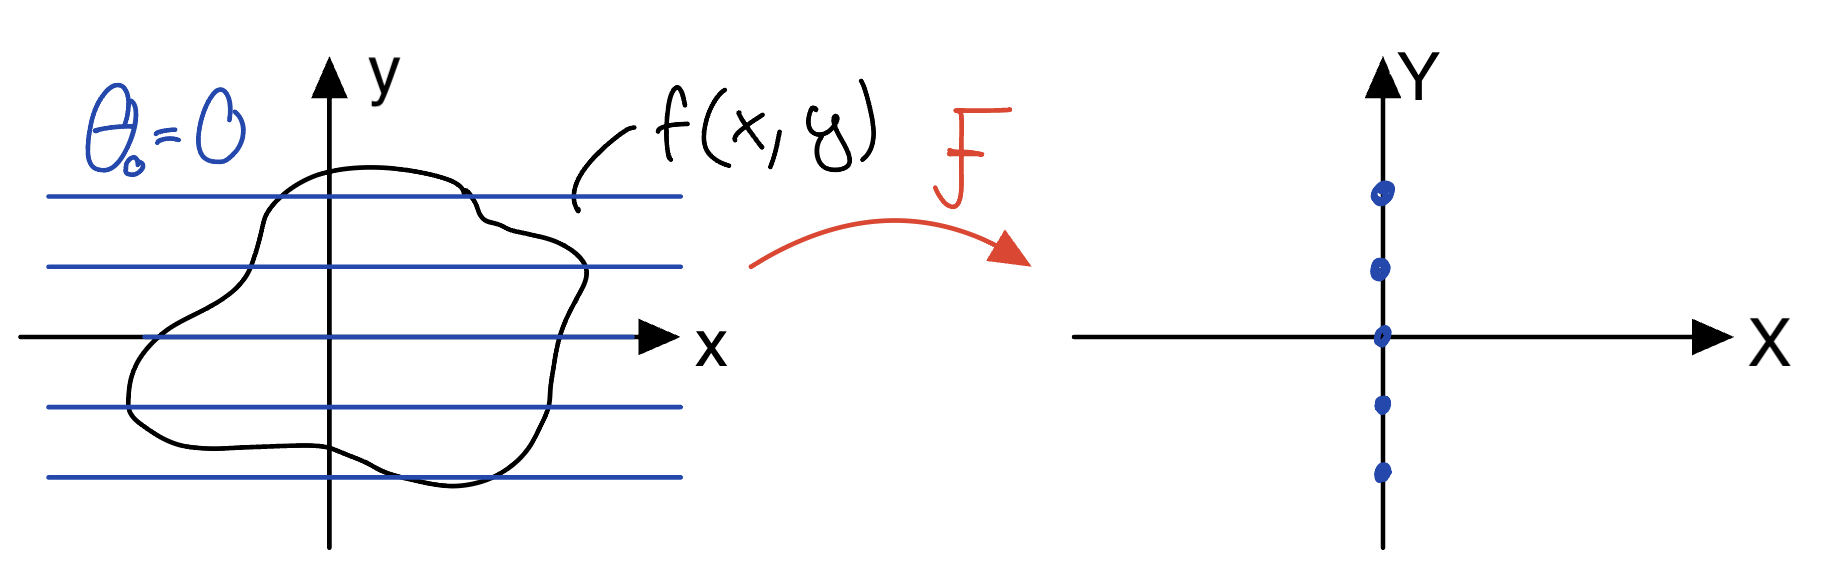
\includegraphics[width=0.35\linewidth]{papers/ct/images/central-slice.png}}
	\subfigure[Beispielbild Radon-transformiert.]{\label{ct:fig:central-slice2}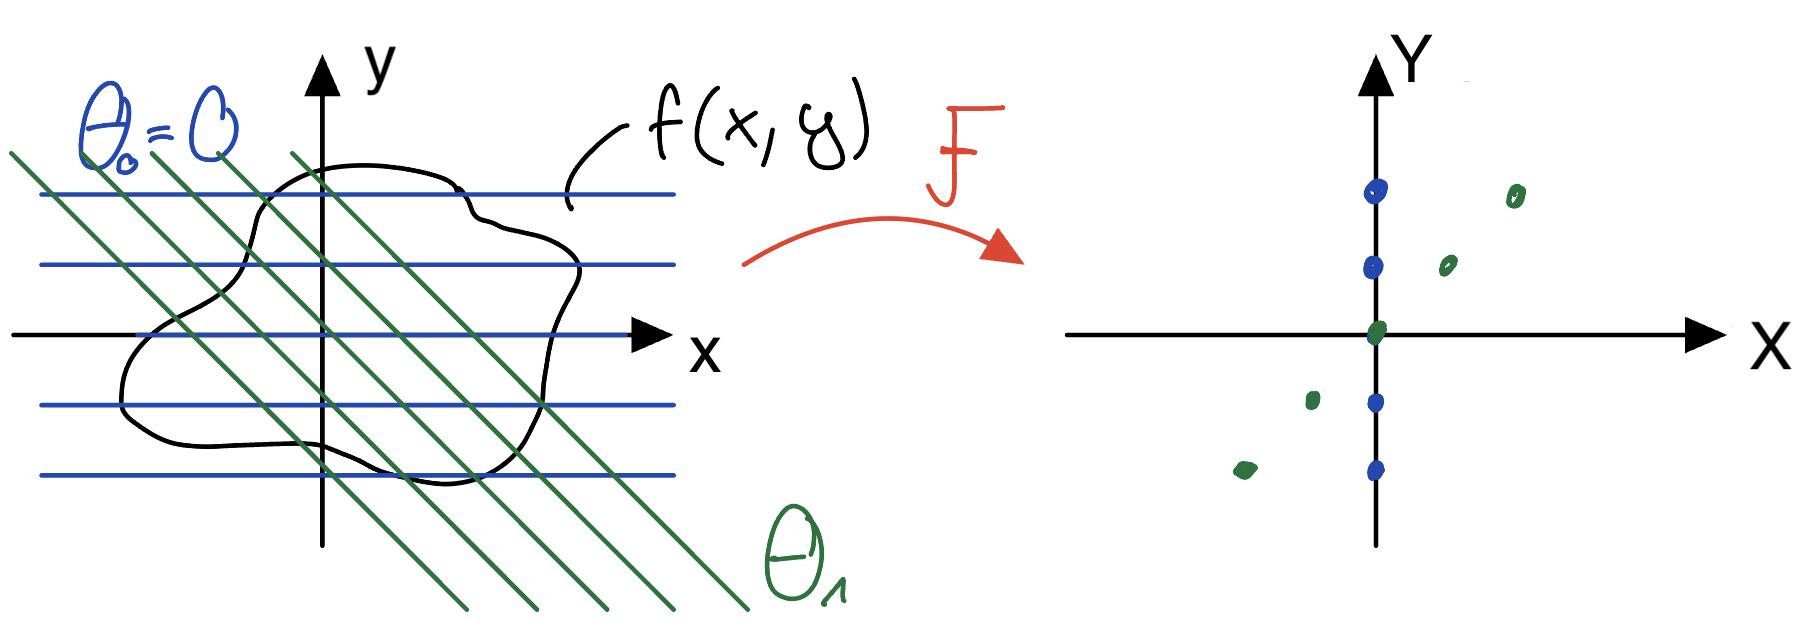
\includegraphics[width=0.55\linewidth]{papers/ct/images/central-slice2.png}}
	\caption{Visualisierung des Zentralschnitt-Theorems.}
\end{figure}


\subsection{Die gefilterte Rückprojektion
	\label{ct:subsection:gefilterterueck}}
Die Rückprojektion diente als erster Versuch, die Radon-Transformation zu invertieren und die Funktion des Dämpfungskoeffizienten zu ermitteln. Das Ergebnis war jedoch eine geglättete Version der ursprünglichen Funktion und keine exakte Übereinstimmung. Das nachfolgende Theorem, das als gefilterte Rückprojektion bekannt ist, zeigt eine Methode zur Korrektur des Glättungseffekts und zur genauen Wiederherstellung der ursprünglichen Funktion.

Die gefilterte Rückprojektion besagt, dass für eine geeignete Funktion $f$, die in einer Ebene definiert ist und für reelle Zahlen $x$ und $y$ gilt, dass
\begin{equation}
	f(x, y) = \dfrac{1}{2}\mathscr{B}\biggl(\mathscr{F}^{-1}[|S|\mathscr{F}(\mathscr{R}f(S, \theta))]\biggr)(x,y).
\end{equation}

Als nächstes folgt der Beweis für die gefilterte Rückprojektion.
\begin{proof}[Beweis]
	Wird die (2-dimensionale) Fourier-Transformation und die Inverse-Fourier-Transformation auf eine Funktion $f$ angewendet, resultiert 
	\begin{align}\label{iftnft}
		f(x, y) &=\mathscr{F}_2^{-1} \mathscr{F}_2 f(x, y). \\
		\intertext{	Wird die Definition der inversen 2-dimensionalen Fourier-Transformation auf der rechten Seite der Gleichung angewendet, folgt dass}
				&=\dfrac{1}{4\pi^2} \int_{-\infty}^{\infty}\int_{-\infty}^{\infty} \mathscr{F}_2 f(x, y)e^{+i(xX + yY)}\,dX\,dY. \\
		\intertext{Danach wird eine Koordinaten-Transformation von Kartesischen- zu Polarkoordinaten durchgeführt, wobei $X = S\cos(\theta)$ und $Y = S\sin(\theta)$. Dabei ist $S$ auf reelle Zahlen und $\theta$ auf den Bereich $0 \le \theta \le \pi$ beschränkt. Angesichts dieser Änderung resultiert für $dX\,dY = |S|\,dS\,d\theta$, anstatt $S\,dS\,d\theta$. Dies führt dazu, dass}
				&= \dfrac{1}{4\pi^2} \int_{0}^{\pi}\int_{-\infty}^{\infty} \mathscr{F}_2 f(S\cos(\theta), S\cos(\theta))e^{+iS(x\sin(\theta) + y\sin(\theta))}\,|S|\,dS\,d\theta \\
		\intertext{	resultiert. Aus dem Zentralschnitt-Satz folgt für den Integrand $\mathscr{F}_2 f(S\cos(\theta), S\cos(\theta))$, dass dies das Gleiche ist wie $\mathscr{F}(\mathscr{R}f)(S, \theta)$. Somit kann auch geschrieben werden, dass}
				&= \dfrac{1}{4\pi^2} \int_{0}^{\pi}\int_{-\infty}^{\infty} \mathscr{F}(\mathscr{R}f)(S, \theta)e^{+iS(x\sin(\theta) + y\sin(\theta))}\,|S|\,dS\,d\theta.\\
		\intertext{Das innere Integral in Bezug auf $S$ ist definiert, als das $2\pi$-fache der inversen Fourier-Transformation der Funktion $|S|\mathscr{F}(\mathscr{R}f)(S, \theta)$ ausgewertet am Punkt $(x\cos(\theta) + y\sin(\theta), \theta)$. Dies führt dazu, dass }
				&= \dfrac{1}{2\pi} \int_{0}^{\pi} \mathscr{F}^{-1}[|S|\mathscr{F}(\mathscr{R}f)(S, \theta)](x\cos(\theta)+y\sin(\theta), \theta)\,d\theta.\\
		\intertext{\sloppy Dies ist wiederum das Integral, welches auch für die gefilterte Rückprojektion der Funktion $\mathscr{F}^{-1}[|S|\mathscr{F}(\mathscr{R}f(S, \theta))]$ verwendet wird. Deshalb entspricht auch}
		f(x, y) &= \dfrac{1}{2}\mathscr{B}\biggl(\mathscr{F}^{-1}[|S|\mathscr{F}(\mathscr{R}f(S, \theta))]\biggr)(x,y),
	\end{align}
	womit die gefilterte Rückprojektionsformel erfolgreich eingeführt wurde.
\end{proof}

Würde in der Formel der Faktor $|S|$ fehlen, würden sich die Fourier-Transformation und ihre Umkehrung gegenseitig aufheben, so dass nur die Rückprojektion der Radon-Transformation von $f$ übrig bliebe. Wenn man die 1-dimensionale Fouriertransformierten für verschiedene Winkel aufaddiert, dann werden bei tiefen Frequenzen viele Werte zusammengezählt, bei hohen Frequenzen nur wenige. Dieser Effekt wird ausgeglichen durch Multiplikation mit dem Betrag der Frequenz entlang der Frequenzachse $\omega$. Das entscheidende Element in der Formel besteht also darin, die Fourier-Transformierte von $\mathscr{R}f(S, \theta)$ mit der Absolutwertfunktion $|S|$ zu multiplizieren, bevor die inverse Fourier-Transformation durchgeführt wird. Im Kontext der Signalverarbeitung wird die Fourier-Transformation von $\mathscr{R}f$ als gefiltert durch Multiplikation mit $|S|$ beschrieben. Genau aus diesem Grund wird die Formel auch als \glqq gefilterte Rückprojektionsformel\grqq{} bezeichnet.

Die Formel für die gefilterte Rückprojektion dient als Basis der Bildrekonstruktion. Sie beruht jedoch auf der Annahme, dass die Werte von $\mathscr{R}f(S, \theta)$ für alle möglichen Geraden $l_{S, \theta}$ bekannt sind. In der Praxis ist dies nicht möglich, da nur eine endliche Anzahl von Röntgenproben genommen wird und ein Bild aus den gesammelten Daten approximiert werden muss. Folglich gibt es für jede endliche Menge von Röntgenstrahlen, die einen Scan bilden, von Null abweichende Dämpfungskoeffizientenfunktion, die als Artefakte bezeichnet werden und deren Radon-Transformationen für alle Zeilen des Scans zu Null werden.





















%
% teil3.tex
%
% (c) 2023 Vincent Haufe, Hochschule Rapperswil
%
% !TEX root = ../../buch.tex
% !TEX encoding = UTF-8
%
\section{Vergleich mit der Fouriertransformation
\label{mellin:section:teil3}}
\rhead{Teil 3}
Im vorangehenden Abschnitt wurde die Mellin-Transformation aus den 
Regeln der Gelfandtheorie konstruiert. 
Dabei wurde auch immer wieder auf die bekannte Fouriertransformation 
verwiesen und deren Parallelen gezogen, um die doch sehr abstrahierte 
Theorie etwas zu bodigen.
Das hat dabei in diesem Fall besonders gut funktioniert, da die Fourier- 
und Mellin-Transformation nämlich nicht nur beide eine generische 
Gelfandtransformation sind, sondern auch untereinander enger verwandt 
sind als prinzipiell nötig wäre.
Der folgende Abschnitt erkundet eine Alternative, wie man auf die 
Mellin-Transformation auf sehr einfache Weise auch direkt vom Integral 
der Fouriertransformation hätte kommen können.

\subsection{Von Fourier zu Mellin
\label{mellin:subsection:foumel}}
Was folgt ist eine einzelne Rechnung.
Wir starten mit dem bekannten Integral der Fouriertransformation
\begin{equation}
    \mathcal{F}\{f \}(\omega) = 
    \int\limits_{-\infty}^{\infty} e^{-j\omega{}t} f(t) \,\mathrm{d}t
    \label{mellin:fourier}
\end{equation}
Jetzt gilt es, zwei Substitution durchzuführen
\begin{align*}
    -j\omega &= z
\end{align*}
und
\begin{align*}
    t &= \ln x \\
    \mathrm{d}t &= \frac{1}{x} \mathrm{d}x
\end{align*}
Eingesetzt in das Fourier-Integral ergibt sich
\begin{align*}
    \int e^{z \ln x} \cdot f(\ln x) \,\frac{\mathrm{d}x}{x}
    = &\int e^{\ln x^z} \cdot f(\ln x) \,\frac{\mathrm{d}x}{x} \\
    = &\int x^{z} \cdot f(\ln x) \,\frac{\mathrm{d}x}{x} \\
    = &\int x^{z-1} \cdot f(\ln x) \,\mathrm{d}x \\
\end{align*}
Nun gilt es bei der Substitution der Integrationsvariablen $t$ noch die 
neuen Grenzen zu berechnen
\begin{align*}
    e^{t} &= x \\
    e^{-\infty} &\rightarrow 0 \\
    e^{\infty} &\rightarrow \infty 
\end{align*}
Dies führt auf das Integral
\[
    \int\limits_{0}^{\infty} x^{z-1} f(\ln x) \,\mathrm{d}x
\]
Das nun bekannt vorkommen sollte, denn es entspricht exakt der 
Mellin-Transformation!
\medskip

Die Fouriertransformation einer Funktion ist also dasselbe wie die 
Mellin-Transformation derselben Funktion, welche aber mit dem natürlichen 
Logarithmus logarithmiert wurde, oder andersherumn, nimmt man das 
Argument einer Funktion in den Exponent von $e \mapsto e^x$ und 
fouriertransformiert diese, ergibt dies die Mellin-Transformation 
der Funktion $f(x)$.
Dies rührt daher, da die Exponentialfunktion eine Funktion von 
$\mathbb{R} \mapsto \mathbb{R^+}$ ist.
Das ist eine erstaunliche Erkenntnis und lässt ein paar einfache 
Relationen zur Fourier- und Laplace-Transformation formulieren.
\begin{align*}
    \mathcal{M}\left\{f(x)\right\}(z) 
    &= \mathcal{F}\left\{f (e^{t})\right\}(jz) \\ \\
    \mathcal{M}\left\{f(x)\right\}(z) 
    &= \mathcal{L}\left\{f (e^{-t})\right\}(-z) 
    + \mathcal{L}\left\{f (e^{t})\right\}(z) 
\end{align*}
und
\begin{align*}
    \mathcal{M}^{-1}\left\{f(z)\right\}(x) 
    &= \mathcal{F}^{-1}\left\{f (jz)\right\}(e^t) \\ \\
    \mathcal{M}^{-1}\left\{f(z)\right\}(x) 
    &= \mathcal{L}^{-1}\left\{f (-z)\right\}(e^{-t}) 
    + \mathcal{L}^{-1}\left\{f (z)\right\}(e^{t}) 
\end{align*}
Aus diesen Relationen können also Hin- und Rücktransformationsformeln 
der Mellin-Transformation einfachst aus den Formeln der Fourier- oder 
Laplacetransformation hergeleitet werden, ganz ohne Kenntnis der 
zugrundeliegenden Gruppen- beziehungweise Gelfandtheorie.
Auch überrascht nun gar nicht mehr, dass eigentlich alle Eigenschaften 
der Fouriertransformation übersetzt werden können, was vorher im Kontext 
der abstrakten Gelfandtheorie vielleicht noch etwas undurchsichtig 
erschienen ist.

In der Theorie könnte die Mellin-Transformation also alle Aufgaben der 
in der modernen Welt allgegenwärtigen Fouriertransformation übernehmen. 
Joseph Fourier hätte die Wärmeleitgleichung damals ebenso mit der 
Mellin-Transformation lösen können und ein Grossteil der modernen 
Elektrotechnik könnte darauf basieren. 
Aus diesem Vergleich offenbart sich aber auch die Schönheit der 
Fouriertransformation. 
Durch die Symmetrie der Gruppen und dadurch der Transformationsgleichungen 
kommt diese extrem handlich und intuitiv daher und ist der 
Mellin-Transformation in dieser Hinsicht wohl doch überlegen.
Die Vorstellung der Fouriertransformation, als das Aus- und 
Einrollen eines Seiles in einer Seiltrommel ist in diesem Kontext 
einzigartig.
% to be elaborated





\printbibliography[heading=subbibliography]
\end{refsection}
